%-------------------------------------------------------------------------------
\section{Countermeasure} \label{sec:countermeasure}
%-------------------------------------------------------------------------------
% In this section, we xxxx.

In this section, we analyze the causes of order tampering attacks, introduce our countermeasure, verify it using symbolic methods, and discuss it.

\subsection{Cause Analysis}

\textbf{Superficial Causes.}
From a superficial perspective, order tampering attacks arise from insecure communication channels between \emph{MS} and \emph{PS-App}, over which an attacker can tamper with order information and mislead the user into authorizing an incorrect payment.
Securing these channels is difficult for payment service providers in practice: the path from merchant backends to \emph{PS-App} depends on the backend implementations of a large number of merchants and on the network environments of a vast user base, both of which lie beyond the providers' control.
Consequently, mitigation is often reactive: once an insecure communication channel is identified, merchants and users are notified to apply patches.

\textbf{Root Causes.}
The root cause of such attacks lies in the lack of a user-side authentication mechanism for order information in existing payment patterns.
During payment, the user enters a payment password to authorize the transaction and possibly checks the payment amount and description.
These values describe the content of the current payment, not the original order that the user intends to confirm, so the user's authorization applies only to the act of payment rather than to a specific order.
Once an attacker is able to tamper with order parameters in transit, the user can be induced to authorize an incorrect order.

An order created through the order oracle carries the same amount, description, and payee as the user's order, so it passes every check the user performs; the two orders differ only in the order instance and in the party that receives the goods.
\emph{PS} cannot tell them apart either, because it cannot authenticate the sender of the payment parameters, so a countermeasure has to give the user a check that the attacker cannot reproduce with its own order.

\subsection{Design Goals}

We design the countermeasure to meet four goals.
\begin{enumerate}[leftmargin=*, label=\textbf{G\arabic*}]
  \item \textbf{Protection of every payment.} The first payment between a user and a merchant is protected in the same way as every later payment.
  \item \textbf{Single round and no per-user state.} A payment completes in one run of the protocol, without per-user keys, locally stored bindings, or trust decisions by the user.
  \item \textbf{Compatible integration.} Merchants keep the existing prepayment and notification interfaces.
  \item \textbf{Weak channel assumptions.} Security holds when both \emph{MF} $\Longleftrightarrow$ \emph{MS} and \emph{MF} $\Longleftrightarrow$ \emph{PS} are insecure.
\end{enumerate}
Our countermeasure, Sealed Checkout Code (SCC), meets all four goals.

\subsection{Countermeasure Design}

\begin{figure}[t]
  \centering
  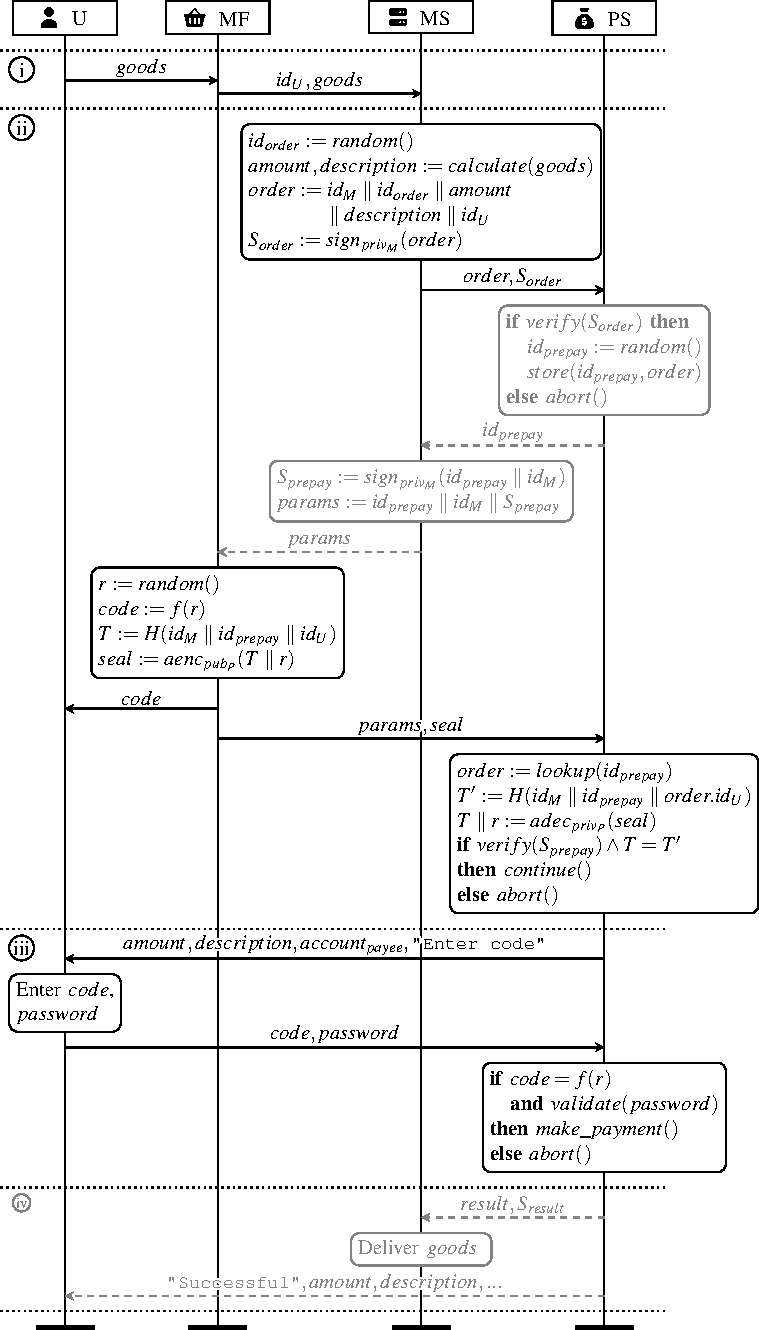
\includegraphics[width=0.85\linewidth]{img/cm_scc.pdf}
  \caption{Sealed Checkout Code on top of payment pattern~B.
    Black elements are new or changed; gray elements are identical to pattern~B.
    Notation: $D$ denotes the fulfilment target of the order; $H$ denotes a hash function; $aenc_{k}(m)$ and $adec_{k}(c)$ denote public-key encryption and decryption; $f$ maps a nonce to a short code; $lookup(id_{prepay})$ returns the order that \emph{PS} recorded for $id_{prepay}$.}
  \label{fig:cm_scc}
\end{figure}

SCC uses the user as the link between \emph{MF} and \emph{PS} that the attacker does not control.
For each payment, \emph{MF} draws a fresh nonce $r$, seals it to \emph{PS} together with a digest of the order handle and the fulfilment target, and shows a short code derived from $r$ to the user.
\emph{PS} opens the seal only for the order it was created for, and completes the payment only if the user enters the same code.
Fig.~\ref{fig:cm_scc} shows the workflow on top of payment pattern~B.

\textbf{Fulfilment target.}
The fulfilment target $D$ is the information that determines who receives the goods, such as a shipping address, a recipient, a mobile number to top up, or a game account.
The user enters or selects $D$ in \emph{MF} at checkout, so the value held by \emph{MF} comes from the user over a secure channel.

\textbf{Order Phase.}
The user selects $goods$ and $D$ in \emph{MF}, and \emph{MF} sends $id_{U}$, $goods$, and $D$ to \emph{MS}.

\textbf{Prepayment Phase.}
\emph{MS} includes $D$ in the order it signs and submits to \emph{PS}, and \emph{PS} records the order under a fresh $id_{prepay}$.
\emph{MS} then generates the payment parameters exactly as in pattern~B.
Upon receiving the parameters, \emph{MF} draws $r$, computes $code = f(r)$ and $T = H(id_{M} \parallel id_{prepay} \parallel D)$ with the $D$ entered by the user, and encrypts $T \parallel r$ under the public key $pub_{P}$ of \emph{PS} to obtain $seal$.
\emph{MF} displays $code$ to the user and sends the payment parameters together with $seal$ to \emph{PS}.
\emph{PS} verifies $S_{prepay}$, looks up the order recorded for $id_{prepay}$, recomputes $T'$ from the merchant identifier, the order handle, and the fulfilment target in that order, and decrypts $seal$.
It continues only if $T = T'$.

\textbf{Authorization Phase.}
\emph{PS-App} displays the amount, the description, and the payee account, and asks the user to enter the code.
The user enters the code shown by \emph{MF} together with the payment password, and \emph{PS} completes the payment only if the code equals $f(r)$ and the password is valid.

\textbf{Notification Phase.}
This phase is identical to pattern~B, and \emph{MS} fulfils the order to $D$.

\textbf{Direction of the code.}
\emph{PS} never displays the code.
Payment parameters are bearer tokens: any party holding them can open the cashier.
If \emph{PS-App} displayed the code for the user to compare, an attacker that intercepts the parameters and the seal could open the cashier under its own payment account, read the code, and choose a nonce $r_A$ with $f(r_A)$ equal to that code for its own order.
In SCC the code travels only from \emph{MF} to the user and from the user to \emph{PS}, both over secure channels.

\textbf{Integration.}
Merchants integrate SCC by adding $D$ to the signed order.
The seal and the code are computed by the payment SDK embedded in \emph{MF}, which also carries $pub_{P}$, and the prepayment and notification interfaces remain unchanged.

\subsection{Security Analysis}

The attacker controls \emph{MF} $\Longleftrightarrow$ \emph{MS} and \emph{MF} $\Longleftrightarrow$ \emph{PS} and obtains legitimate payment parameters for its own orders through the order oracle.
To make the user pay for an order of its own, the attacker has three options.

\begin{enumerate}[leftmargin=*]
  \item \textbf{Substitute its own order.}
  The attacker replaces the user's payment parameters with those of its own order, either on \emph{MF} $\Longleftrightarrow$ \emph{MS} (Variant~\Rom{1}) or on \emph{MF} $\Longleftrightarrow$ \emph{PS} while keeping the user's seal (Variant~\Rom{2}).
  In Variant~\Rom{1}, \emph{MF} seals the attacker's order handle together with the user's $D$; in Variant~\Rom{2}, the seal carries the user's order handle.
  \emph{PS} recomputes $T'$ from the attacker's order, which carries the attacker's own handle and fulfilment target, so $T \neq T'$ and \emph{PS} aborts.
  \item \textbf{Forge a seal for its own order.}
  The attacker builds a consistent seal for its own order with a nonce $r_A$ of its choice.
  \emph{PS} opens the cashier, but the payment requires $f(r_A)$, while the user enters the code $f(r)$ shown by its own \emph{MF}.
  The nonce $r$ appears only inside the seal and as the code on the channel between \emph{MF} and the user, so the attacker can only guess.
  With a four-digit code, a guess succeeds with probability $10^{-4}$, and \emph{PS} bounds the number of failed attempts per payment.
  \item \textbf{Tamper with the fulfilment target.}
  The attacker changes $D$ on its way to \emph{MS}.
  The order at \emph{PS} then carries the attacker's target while \emph{MF} seals the user's target, so $T \neq T'$ and the payment fails.
\end{enumerate}

In every case the attack ends with a failed payment and does not redirect the user's funds or goods.

\subsection{Symbolic Verification}


\begin{table}[t]
\centering
\small
\setlength{\tabcolsep}{5pt}
\renewcommand{\arraystretch}{1.12}

\caption{Verification Results of Countermeasure. \textcolor{xgreen}{\ding{51}}~indicates that the security property is satisfied.}
\label{tab:countermeasure-results}

\begin{tabularx}{\linewidth}{Xccccc  >{\raggedright\arraybackslash}X }
\toprule
\textbf{Protocol} &
\textbf{IA-O1} & \textbf{IA-O2} & \textbf{IA-UA} & \textbf{IA-R1} & \textbf{IA-R2} & \textbf{Time (s)} \\
\midrule

SCC & \textcolor{xgreen}{\ding{51}}  & \textcolor{xgreen}{\ding{51}}  & \textcolor{xgreen}{\ding{51}} & \textcolor{xgreen}{\ding{51}} & \textcolor{xgreen}{\ding{51}}  & 454.94\\

\bottomrule
\end{tabularx}

\end{table}

We model SCC in \Tamarin following the countermeasure models of our artifact, with the same channel rules, query oracle, tactics, and lemmas.
The model uses the Base assumption, in which both \emph{MF} $\Longleftrightarrow$ \emph{MS} and \emph{MF} $\Longleftrightarrow$ \emph{PS} are insecure; it grants the attacker the capabilities of both SecureMS and SecurePS.
Through the order oracle, the attacker places orders with arbitrary amounts and descriptions on its own account, and each such order carries the attacker's own fulfilment target, consistent with the merchant's record of the order.

The user commits to the order when the payment completes, because \emph{PS} checks the code after the user submits it.
To confirm that this commit point preserves the discriminating power of IA-O2, we applied the same change to all six protocols of Table~\ref{tab:lemma-results} under all three channel assumptions; IA-O2 remains falsified in all 18 models.

Table~\ref{tab:countermeasure-results} summarizes the results.
SCC satisfies all five security properties under the Base assumption.
The verification used \Tamarin version~1.10.0 on a server with 32 CPU cores and 187~GB of memory (peak usage 7.0~GB).
